\subsubsection{Data Driven QCD and $\gamma$jet}
\label{subsubsec:QCDDataDriven}

For this final state category, a data-driven QCD$+\gamma$jet estimation is performed in a control region where one photon candidate fails the requirement of photon ID $>$ -0.7, previously used and described in \cite{Sirunyan:2020sum}.

% This is shown in Figure \ref{fig:FH_preQCDEstimation_DataMC_photonIDDescription}, as there is a large under

% in a similar manner as perfomed for the ttH analysis in \href{https://cms.cern.ch/iCMS/analysisadmin/cadilines?line=HIG-19-013&tp=an&id=2281&ancode=HIG-19-013}{HIG-19-013}~\cite{Sirunyan:2020sum}. 

% This method is described briefly here and for details please check \cite{Sirunyan:2020sum}.

% At pre-selection level, the dominant background in the Fully-Hadronic channel are QCD multijet production in assosciation with zero to two prompt photons (``QCD + X''), composing $\approx 99\%$ of the background. However, as Fig.~\ref{fig:FH_preQCDEstimation_DataMC_photonIDDescription}(a) shows, there is a large under prediction from MC. The under prediction comes primarily from the lower region of minimum photon ID MVA\footnote{The minimum value of the photon MVA score out of the two selected photons.}, where QCD and $\gamma$ + jets MC samples do not provide an accurate description of fake photons.

% \begin{figure}[H]
%   \setcounter{subfigure}{0}
%   \centering
%   \subfloat[]{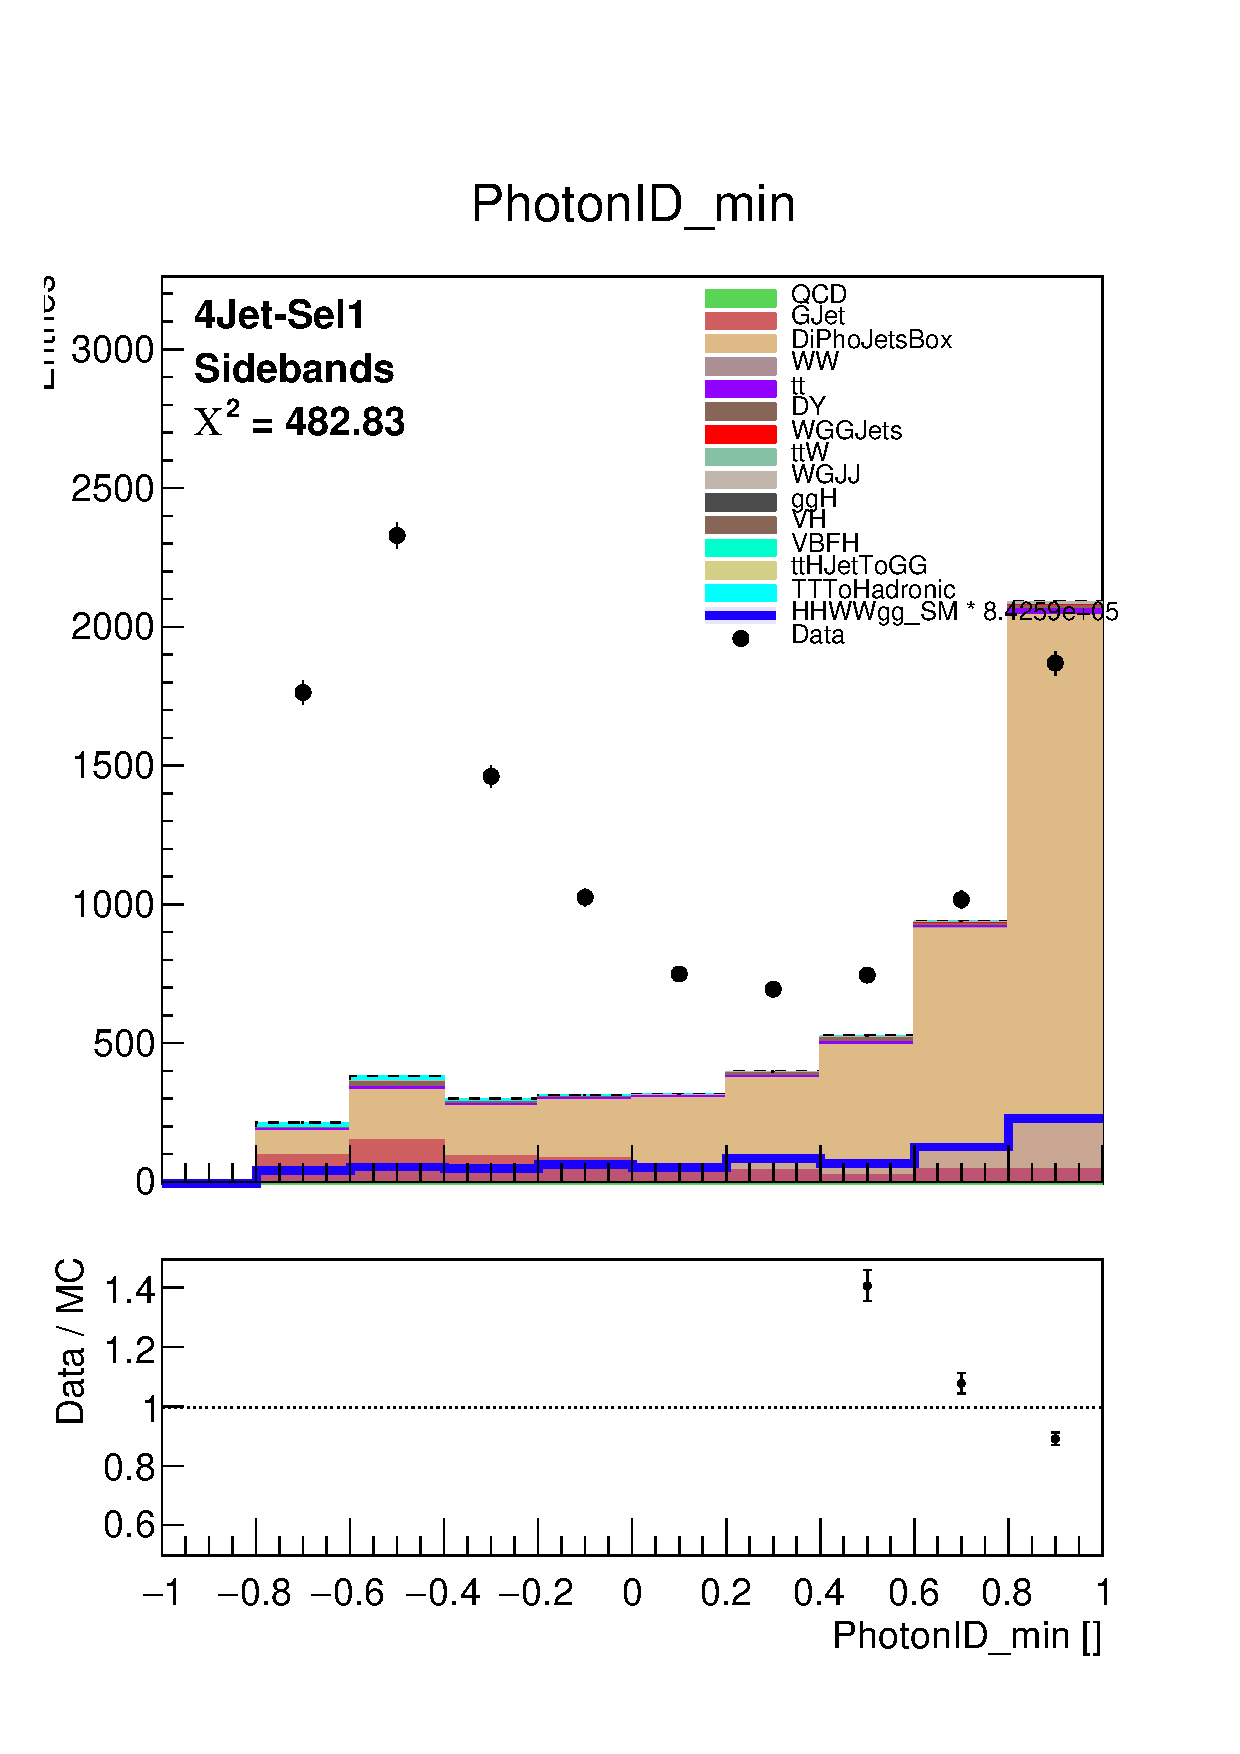
\includegraphics[width=0.45\textwidth]{Sections/HHWWgg/images/FH_DNN/DataDrivenQCD/DataMC_PhotonID_min_SB_nonLog.pdf}}
%   \qquad
%   \subfloat[]{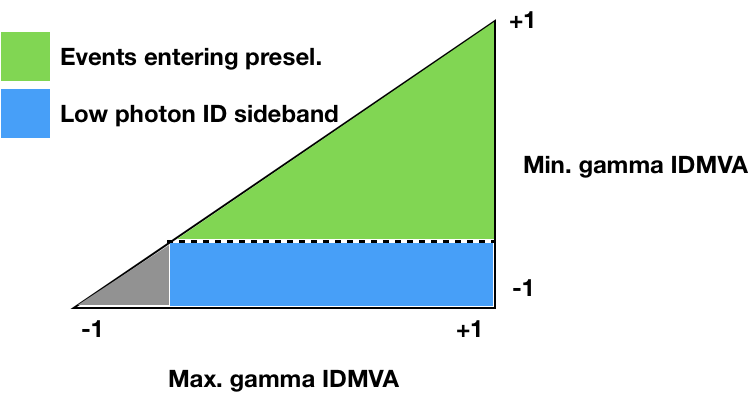
\includegraphics[width=0.45\textwidth]{Sections/HHWWgg/images/FH_DNN/DataDrivenQCD/figures_impute_photonID_diagram.png}} %%-- as of 6 Sep 2021, missing this image on gitlab 
%   \caption{(a) Minimum Photon ID MVA. (b) Diagram of the Loose MVA pre-selection (green) and the Low Photon ID Sideband (blue).}
%   \label{fig:FH_preQCDEstimation_DataMC_photonIDDescription}
% \end{figure}

% The data-driven description is obtained by using the events which fail the pre-selection cut on minimum $\gamma$ ID MVA (-0.7) in place of events from QCD and $\gamma$ + jets MC samples. This region is referred to as the ``low photon ID sideband'', as shown in Fig.~\ref{fig:FH_preQCDEstimation_DataMC_photonIDDescription}(b).

% The overall normalization of events from the low photon ID sideband should not be expected, a priori, to be the same as the number of QCD and $\gamma$+jets events in the pre-selection. To address this, a simultaneous fit in the minimum and maximum photon ID MVA is performed to obtain the scale factor. This is shown in Tab.~\ref{tab:FH_QCD_gg_SF}.
% \begin{table}[!htbp]
%     \centering
%     \begin{tabular}{|l||r|} \hline
%     Template & Scale \\ \hline
%     QCD (data driven) & 0.9 \\ \hline
%     $\gamma \gamma $+jets & 1.25 \\ \hline
%     \end{tabular}
%     \caption{Scale factor obtained from a simultaneous fit of data to MC of the minimum photon ID and maximum photon ID distributions}
%     \label{tab:FH_QCD_gg_SF}
% \end{table}

% To check our estimated background, the QCD and $\gamma$+jets MC was replaced with the data-driven background using appropriate SF given in Tab.~\ref{tab:FH_QCD_gg_SF}, the data/MC comparison was performed and shown in Fig.~\ref{fig:FH_DataMC_1}
% , ~\ref{fig:FH_DataMC_2}, ~\ref{fig:FH_DataMC_3}, and ~\ref{fig:FH_DataMC_4}. This shows that the data/mc comparison improved a lot after this estimation.